\section{Consensus layer support} \label{sec:consensus}

\todo{Include interlink-set data structure also}

\subsection{The interlink pointers data structure}
\label{sec:interlink}

In order to construct our protocol, we rely on the \emph{interlink data
structure}~\cite{popow}. This is an additional hash-based data
structure that is proposed to be included in the header of each block. The
interlink data structure is a skip-list~\cite{skiplist} that makes it efficient
for a verifier to process a sparse subset of the blockchain, rather than only
consecutive blocks.

Valid blocks satisfy the proof-of-work condition: $id \leq T$, where $T$ is the
mining target. In this chapter, we work in the static difficulty, and so make
the simplifying assumption that $T$ is constant. Some blocks will achieve a
lower id. If $id \leq \frac{T}{2^\mu}$ we say that the block is of level $\mu$.
All blocks are level $0$. Blocks with level $\mu$ are called
$\mu$-\emph{superblocks}. $\mu$-superblocks for $\mu > 0$ are also $(\mu -
1)$-superblocks. The level of a block is given:

\begin{definition}[Level]\index{Level}
  Let $B$ be a valid block. Its \emph{level} $\mu$ is defined as:

  \[
  \mu = \emph{level}(B) = \left \lfloor \log(T) -
\log(\sf{id}(B)) \right \rfloor
  \,.
  \]

  By convention for $Gen$ we set $\mu = \infty$.
\end{definition}

\begin{definition}[Superblock]\index{Superblock}
  A block of level $\mu$ is called a \emph{$\mu$-superblock}.
\end{definition}

Observe that in a blockchain protocol execution it is expected $1/2$ of the
blocks will be of level $1$; $1/4$ of the blocks will be of level $2$; $1/8$
will be of level $3$; and $1/2^\mu$ blocks will be of level $\mu$. In
expectation, the number of superblock levels of a chain $\chain$ will be
$\Theta(\log(\chain))$~\cite{popow}. Figure~\ref{fig.hierarchy} illustrates the
blockchain superblocks starting from level $0$ and going up to level $3$ in case
these blocks are distributed exactly according to expectation. Here, each level
contains half the blocks of the level below.

We wish to connect the blocks at each level with a \emph{previous block}
pointer pointing to the most recent block of the same level. These pointers must
be included in the data of the block so that proof-of-work commits to them. As
the level of a block cannot be prediced before its proof-of-work is calculated,
we extend the \emph{previous block id} structure of classical blockchains to be
a vector, the \emph{interlink vector}\index{Interlink}. The interlink vector
points to the most recent preceding block of every level $\mu$. Genesis is of
infinite level and hence a pointer to it is included in every block. The number
of pointers that need to be included per block is in expectation
$\log(|\chain|)$.

\begin{figure}
    \caption{The hierarchical blockchain.
    Higher levels have achieved a lower target (higher difficulty) during
    mining. All blocks are connected to the genesis block $G$.}
    \centering
    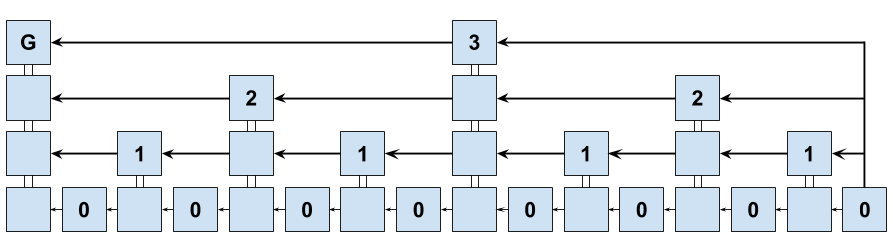
\includegraphics[width=0.7\columnwidth,keepaspectratio]{chapters/work/figures/hierarchical-ledger.png}
    \label{fig.hierarchy}
\end{figure}

The algorithm for this construction is shown in
Algorithm~\ref{alg.nipopow-interlink} and is borrowed from~\cite{popow}. The
interlink data structure turns the blockchain into a
skiplist-like~\cite{skiplist} data structure.

The updateInterlink algorithm accepts a block $B'$, which already has an
interlink data structure defined on it. The function evaluates the
interlink data structure which needs to be included as part of the next block.
It copies the existing interlink data structure and
then modifies its entries from level $0$ to $\textsf{level}(B')$ to
point to the block $B'$.

\begin{algorithm}[H]
    \caption{\label{alg.nipopow-interlink}updateInterlink}
    \begin{algorithmic}[1]
        \Function{\sf updateInterlink}{$B'$}
            \Let{\textsf{interlink}}{B'.\textsf{interlink}}
            \For{$\mu = 0$ to $\emph{level}(B')$}
                \Let{\textsf{interlink}[\mu]}{\textsf{id}(B')}
            \EndFor
            \State\Return{\textsf{interlink}}
        \EndFunction
    \vskip8pt
    \end{algorithmic}
\end{algorithm}


We will only care about \emph{whether} a block contains a pointer to a previous
block, not the positions of these pointers within the block.
An optimization we can readily perform on this algorithm is to treat the
interlink vector as a \emph{set} and remove duplicates, as illustrated in
Algorithm~\ref{alg.interlink-set-update}. This optimization achieves a constant
saving of about $50\%$ in expectation~\cite{compactsuperblocks}.

\begin{algorithm}[H]
    \caption{\label{alg.interlink-set-update}The updateInterlinkSet algorithm which
             updates the interlink set}
    \begin{algorithmic}[1]
        \Function{\sf updateInterlinkSet}{$B'$}
            \Let{\textsf{interlinkSet}}{\{H(B')\}}
            \For{$H(B) \in B'.\textsf{interlink}$}
                \If{$\emph{level}(B) > \emph{level}(B')$}
                    \Let{\textsf{interlinkSet}}{\textsf{interlinkSet} \cup \{H(B)\}}
                \EndIf
            \EndFor
            \State\Return{\textsf{interlinkSet}}
        \EndFunction
    \vskip8pt
    \end{algorithmic}
\end{algorithm}


\noindent\textbf{Traversing the blockchain. }
As we have now extended blocks to contain multiple pointers to previous blocks,
if certain blocks are omitted from the middle of a chain we will obtain a
subchain, as long as the \emph{blockchain property} is maintained (i.e., that
each block must contain an interlink pointer to its previous block in the
sequence).

Blockchains are sequences, so we will use the set notation defined in
Chapter~\ref{chapter:introduction}. We note that, when manipulating blockchains
in this manner, it is important to remember when the blockchain property is
maintained. In particular, $\chain_1 \cup \chain_2$ and $\chain_1 \cap \chain_2$
as well as chains filtered through set-builder notation,
while sequences of blocks, may not always be chains since pointers may be missing.
If $\chain_1[0] = \chain_2[0]$ and $\chain_1[-1]
= \chain_2[-1]$, we say the chains $\chain_1, \chain_2$ \emph{span} the same
block range.

\begin{definition}[Lowest Common Ancestor]\index{Lowest Common Ancestor}
The \emph{lowest common ancestor} of chains $\chain_1$, $\chain_2$ is defined as

\[
\textsf{LCA}(\chain_1, \chain_2) = (\chain_1 \cap \chain_2)[-1]\,.
\]
\end{definition}

It will soon become clear that it is useful to construct a chain containing only
the superblocks of another chain.

\begin{definition}[Upchain]\index{Upchain}
Given $\chain$ and level $\mu$, the \emph{upchain} $\chain\upchain^\mu$ is
defined as $\{B \in \chain: level(B) \geq \mu\}$.
\end{definition}

A chain containing only $\mu$-superblocks is called a
$\mu$\emph{-superchain}. It is also useful, given a $\mu$-superchain $\chain'$
to go back to the regular chain $\chain$. Given chains $\chain' \subseteq
\chain$, the \emph{downchain} $\chain'\downchain\!\!_\chain$ is defined as
$\chain\{\chain'[0]:\chain'[-1]\}$. $\chain$ is the \emph{underlying chain} of
$\chain'$. The underlying chain is often implied by context, so we will simply
write $\chain'\downchain$. By the above definition, the $\chain\upchain$
operator is absolute: $(\chain\upchain^\mu)\upchain^{\mu + i} =
\chain\upchain^{\mu + i}$. Given a set of consecutive rounds $S = \{r, r + 1,
\cdots, r + j\} \subseteq \mathbb{N}$, we define $\chain^S = \{B \in \chain: B
\text{ was generated during } S\}$.
